%1 - What is known

In the biosensor's community most findings and desicions in designed are achived 
through experimental analyses, trial and error procedures. Using
software to assit the design and manufacturing process can play a key role for 
the future of biosensors. In the world of plasmonics there are few softwares that are used 
to study the physics around biosensors.  Among the most known softwares are COMSOL Multiphysics
a proprietary finite-element platform ({\color{red}cite COMSOL Multiphysics® v. 5.2. 
www.comsol.com. COMSOL AB, Stockholm, Sweden. NOT SURE HOW TO ADD THIS TO BIB} ), 
BEM++ ({\color{red}NOT SURE HOW TO CITE}) an open-source Boundary element method
library to solve time-harmonic Maxwell equations in 3D, and 
MNPBEM, an open-source Matlab toolbox for the simulation of metallic nanoparticles that
uses BEM and Hierarchical matrices \cite{Hohenester2018}. Other software, that do
not rely on plasmonics, the biomolecular electrostatic implementation of 
\pygbe \cite{CooperETal2016} allowed the study of ligand molecule orientation 
sensor \cite{CooperClementiBarba2015}.


%2 - What is Unknown, limitations and gaps

Most of these softwares solve full Maxwell equations, causing computational and 
memory expensive runs. Solving full maxwell equations when it is no necessary (long wave range), 
limits also the problem-size that you can run as a user. Another caveat is the
lack of open-source softwares that do not rely on licensed languages. MNPBEM the
open-source Matlab toolbox has recently evolved to a hierarchical
matrices and iterative solver approach reducing the computation time and memory
needs; however, this software relies on a licensed language (Matlab) making its
accesibility restricted. Even though they are able to solve problems in the order
of ten thousands, we cannot ensure that this amount of elements is good enough for 
the geometry size. The lack of grid convergence analysis and error study in most of the 
softwares in the plasmonic community,
{\color{red}(I haven't find any of this in their papers, Chris what do you know about BEM++)}
force the user to believe in the obtained results without knowing their uncertainty. These
limitations prevent the development of a reproducible approach of any results obtained
with these softwares. 

{\color{red} Another limitation that I don't know how to mention is that most softwares
treat the outside medium as a non-lossy medium}

%Limitation: 
%           - Software only study plasmonic assuming a non-lossy medium. 


%limitations - BEM++ {\color{red}Chris any input in this, limitations?}  
%              private are expensive and not accessible, 
%             matlab not free, 
%             no grid convergence analysis or error study, 
%             no reproducible framework 
%             problem size, geometry, and computation time


%Find structural details of analyte and nanoparticle, and the relative position between them.
%Studies that deal with real protein geometry.
%Gap: study this using fast, free-software dependencies and open source computer
%simulations. 


%3 - Burning question, experimental approach, why ours is new and diff (fill the gap)

Experiments suggest that the distance between the nanoparticle and the analyte 
affects the sensitivity of the sensor \cite{HaesETal2004}. However, the processes 
to lead to this conclusions, were trial an error processes. Therefore, there is not
not enough understanding on what is the relation between high dependance on 
sensitivity on distance in biosensors, specifically LSPR biosensors. \pygbe most
recent application \cite{ClementiETal2017} tends to 
bridge that gap providing via simulations, insights to guide the reasearch process.
The latest release of \pygbe extends the software to nanoplasmonics, treating 
localized surface plasmon resonance (LSPR) quasi-statically \cite{MayergoyzZhang2007}.
Localized surface plasmon resonance (LSPR) biosensors measure the shift of 
plasmon resonace frequency in metallic nanoparticles when a target molecules 
binds to it. LSPR is an optical effect see Figure \ref{fig:lspr}, but electrostatics 
makes a good approximation in the long-wavelength limit. In this work we use
PyGBe's approach to study how the LSPR response changes in the presence of a 
biomolecule. To our knowledge, \pygbe is the only open-source software that uses a Tree code 
fast algorithm—O(N logN), for N unknowns, GMRES iterative solver; and hardware 
acceleration on GPUs to compute the extinction cross-sections of arbitrary 
geometries. The software \footnote{\url{https://github.com/barbagroup/pygbe}} is shared 
under the BSD 3-clause license and the development repository is available on 
Github.



\begin{figure}[h] %  figure placement: here, top, bottom, or page
   \centering
   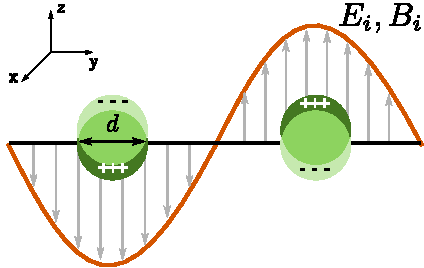
\includegraphics[width=0.35\textwidth]{lspr.pdf} 
   \caption{Localized Surface Plasmon Resonance (LSPR) scheme. LSPR is an 
            optical phenomenon that ocurrs when light shines on conductive 
            nanoparticles that are smaller than the wavelength of the incident 
            light. The free electrons on the surface of the nanoparticle are 
            excited by the incoming electric field oscillating with it and 
            creating plasmons}
   \label{fig:lspr}
\end{figure}


{\color{red} Not sure about where you are taking this introduction.
Perhaps we should discuss a little bit on the point of view of the paper before anything.
We need to be VERY careful about the introduction because it sets the tone, and allows us to highlight what we think is important, but this has to be clear among all authors. 

My impression is that the key result of the paper is that it is the first time that a detailed molecular structure is placed next to the nanoparticle.
The whole discussion on free software, reproducibility, and convergence analysis is interesting, but I don't feel it is central of this paper. 
We've discussed this several times, and even though we know that these topics are extremely important, the rest of the community doesn't necessarily feel that way.
I'm afraid making this the central discussion of the paper might put off editors. 
I would keep the paper more technical.
Plus, we need to be careful not to be looking for everybody else's limitations, rather than focusing on our work.

Plus, I think we should be citing a lot more in the intro. 
I know that Lorena is against loooong literature reviews, and I agree that it shouldn't be that long, but we should be careful, specially if we are ``outsiders'' of the community.

I like the structure of the introduction a lot (known, unknown, fill gap). 
With this structure, what I think the intro should cover is:

What is known:
\begin{itemize}
\item Plasmonic simulations, what applications they cover, etc. (cite Matlab guy, also Garcia de Abajo, Jung+Pedersen, etc. Maybe we can even cite COMSOL here)
\item LSPR: how does it work, what simulations are there in the litarature. Talk about work from, for example, Davis or van Duyne. See page 50 of my thesis (end chapter 2).
\end{itemize}

What is unkown:
\begin{itemize}
\item all developments are trial and error
\item no computational tools to help in the design process
\item example: no understanding of the sensitivity of the system
\item models that consider the nanoparticle and the analyte are extremely simplistic
\end{itemize}

Fill the gap:
\begin{itemize}
\item design of a computational tool that is highly accurate to represent the biomolecule
\end{itemize}

This is just an opinion, though.
We should talk this week to see how you prefer to go about this intro.

}

